% Template for ISBI-2018 paper; to be used with:
%          spconf.sty  - ICASSP/ICIP LaTeX style file, and
%          IEEEbib.bst - IEEE bibliography style file.
% --------------------------------------------------------------------------
\documentclass{article}
\usepackage{spconf,amsmath, amssymb, graphicx}

% Example definitions.
% --------------------
\def\x{{\mathbf x}}
\def\L{{\cal L}}
\newcommand{\etal}{~\textit{et al}.}

% Allow easy processing of labeled images in figures
\newcounter{lfigcounter}
\def\ionbox#1{\makebox[#1]{(\alph{lfigcounter})}\stepcounter{lfigcounter}}
%

% Title.
% ------
\title{Application of Vectorized Persistent Homology Representations for 
Cancer Grading in Digital Histopathology Images}
%
% Single address.
% ---------------
\name{Author(s) Name(s)}%\thanks{Thanks to XYZ agency for funding.}}
\address{Author Affiliation(s)}
%
% For example:
% ------------
%\address{School\\
%	Department\\
%	Address}
%
% Two addresses (uncomment and modify for two-address case).
% ----------------------------------------------------------
%\twoauthors
%  {A. Author-one, B. Author-two\sthanks{Thanks to XYZ agency for funding.}}
%	{School A-B\\
%	Department A-B\\
%	Address A-B}
%  {C. Author-three, D. Author-four\sthanks{The fourth author performed the work
%	while at ...}}
%	{School C-D\\
%	Department C-D\\
%	Address C-D}
%
% More than two addresses
% -----------------------
% \name{Author Name$^{\star \dagger}$ \qquad Author Name$^{\star}$ \qquad Author Name$^{\dagger}$}
%
% \address{$^{\star}$ Affiliation Number One \\
%     $^{\dagger}$}Affiliation Number Two
%
\begin{document}
%\ninept
%
\maketitle
%
\begin{abstract}
% 100 - 150 words
The characterization of glandular structures in histopathology images of adenocarcinomas is a fundamental problem in digital pathology, with important implications for computer-assisted diagnosis and grading. In this paper we describe a new class of features for describing topological patterns in histology images. We describe the mathematical formulation of these features, their implementation, and illustrate their application to colorectal cancer.

\end{abstract}
%
\begin{keywords}
Histopathology, Cancer Diagnosis, Cancer Grading, Persistence homology, Persistence diagrams, Persistence images, Persistence landscapes, Machine learning
\end{keywords}
%
\section{Introduction}
\label{sec:intro}
Histopathology is the study of the presence, extent, and progression of a disease through microscopic examination of thin sections of biopsied tissue that are chemically processed and fixed onto glass slides and dyed with one or more stains to highlight different cellular/tissue components (e.g. cell nuclei or membranes) and antigens/proteins (e.g. Ki-67 indicating cell proliferation) of interest. It is regarded as the gold standard in clinical diagnosis and grading of several diseases including most types of cancer. 

In clinical practice, histologic evaluation still largely depends on manual assessment of glass slides by a pathologist with a traditional microscope, although improvements in whole-slide imaging devices and subsequent regulatory approval of whole-slide-imaging and computational algorithms are rapidly paving the way for increased clinical use of digital imaging and computational interpretation. Algorithmic evaluation of tissue specimens may eventually improve the efficiency, objectivity, reproducibility, and accuracy of the diagnostic process.

Pathologists integrate information across scales from subcellular to macro when evaluating histology. For adenocarcinomas, lesions that originate in the epithelium of glandular structures including lung, prostate, pancreatic, and colorectal cancers, the architecture of glandular structures conveys significant information about the presence and degree of malignancy. Normal appearing structures with organized epithelium become disorganized with the unchecked growth and aberrant signaling in cancer (Figure~\ref{fig:benign_malignant_example}). There have been several efforts to develop quantitative features for characterizing glandular structures for computer-aided grading~\cite{Doyle2007, Doyle2008,Altunbay2010,Singh2014}. In this paper, we present a new set of features based on two recently developed vectorized persistent homology representations called \emph{persistence images} and \emph{persistence landscapes} and demonstrate their application to colorectal cancer grading.

%
\begin{figure*}[t]
\centering
\setcounter{lfigcounter}{1}
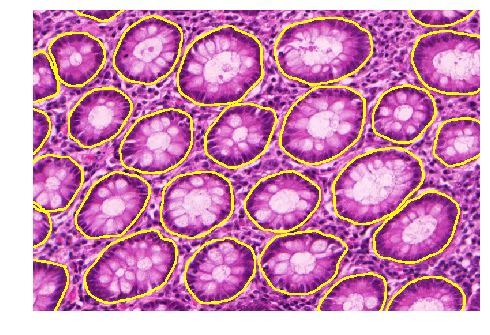
\includegraphics[height=1.2in]{figures/train_22_gland_annot.png}
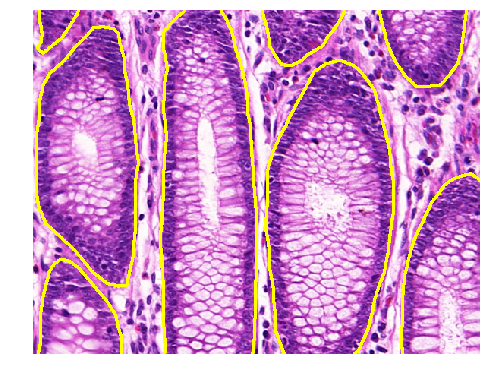
\includegraphics[height=1.2in]{figures/train_84_gland_annot.png}
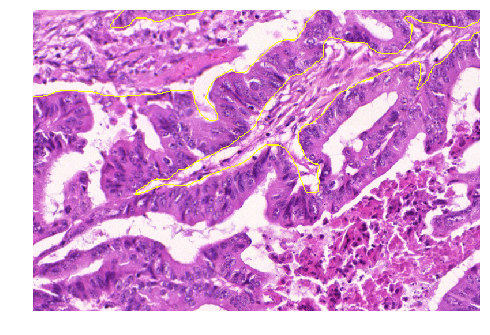
\includegraphics[height=1.2in]{figures/train_11_gland_annot.png}
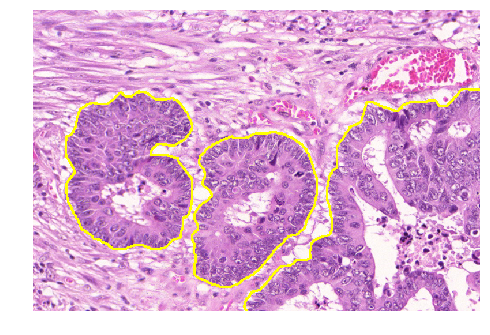
\includegraphics[height=1.2in]{figures/train_81_gland_annot.png}\\
\ionbox{3.0in}\ionbox{3.0in}
\caption{Sample benign (a) and malignant (c) images overlaid (yellow) with manually annotated gland boundaries.}
\label{fig:benign_malignant_example}
\end{figure*}
%
\section{Background}
\label{sec:background}
In this section, we present a brief background on persistence homology. Given a dataset representable in the form of a point cloud in some space, persistent homology can be seen as a theoretical tool to detect and characterize its prominent topological features (e.g. connected components, loops, voids) at multiple scales~\cite{Zhu2013}. These topological descriptors can then be used as features for building machine learning models to solve predictive problems. 

\smallskip
\noindent \textbf{Simplicial homology:} The foundational concepts of persistent homology are simplices, simplicial complexes, filtration, and homology groups. A p-simplex $\sigma_p$ is defined as the convex hull of $p+1$ affinely independent points/vertices. For example, a single vertex is called a 0-simplex, an edge is called a 1-simplex, a triangle is called a 2-simplex, a tetrahedron is called a 3-simplex, and so on. A face of a p-simplex is defined as a subset of its $p+1$ points/vertices. For example, the tetrahedron which is a 3-simplex has 4 triangular faces, 6 edge faces, and 4 vertex faces each of which are simplices themselves. A simplicial complex $K$ is a finite collection of simplices subject to two conditions: (i) if a simplex $\sigma$ is in $K$ and any face of $\sigma$ is also in $K$, and (ii) if two simplices $\sigma$ and $\sigma'$ are in K then $\sigma \cap \sigma'$ must either be empty or a face of both $\sigma$ and $\sigma'$ i.e. they must either be glued together along whole faces or be separate. Given a simplicial complex $K$, a simplicial complex $L$ formed by a subset of its simplices is referred to as the sub-complex of $K$ denoted symbolically as $L \subset K$. A nested sequence of simplicial sub-complexes $K_0 = \phi \subset K_1 \subset K_2 \subset ... \subset K_n = K$ that ascends from an empty set all the way up to $K$ is called a filtration of $K$ denoted as $\mathbb{F}(K)$. A d-dimensional homology group $H_d(K)$ of a simplicial complex $K$ is the set of all d-dimensional holes in it. For example, the 0-dimensional homology group $H_0(K)$ is the set of all connected components, the 1-dimensional homology group $H_1(K)$ is the set of all 2D loops, the 2-dimensional homology group $H_2(K)$ is the set of all 3D cavities and so on. The rank or the number of holes in a d-dimensional homology group $H_d(K)$ is referred to as the d-dimensional Betti number $\beta_d(K)$. 

\smallskip
\noindent \textbf{Vectoris-rips filtration:} Given a dataset in the form of a point cloud of $n$ points $x_1, x_2, ..., x_n \in \mathbb{R}^d$, how can we derive a simplicial complex that encodes the underlying topological structure? One approach for generating it is to examine all subsets of $p+1$ points, and add the p-simplex made up of those points to the simplical complex if the distance between all pairs of points in the simplex is less than a present distance $\epsilon$. Such a complex is called a Vectoris-Rips complex of diameter $\epsilon$ which we will henceforth denote as $VR(\epsilon)$. Note that, if a simplex is in $VR(\epsilon)$, then all its faces are also in $VR(\epsilon)$. The schematic below shows the Vectoris-rips complex for different diameter values for a dataset of four points corresponding to the corners of a rectangle with a width of 2 and height of 1.
\vspace{-0.2cm}
%
\begin{figure}[!h]
\centering
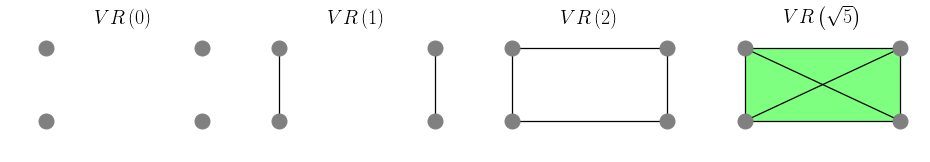
\includegraphics[width=3.5in]{figures/vrcomplex-diagram.png}
\end{figure}
%

\noindent A natural question that arises now is how to choose the best diameter $\epsilon$ for a given dataset. Persistent homology examines all diameters within a range of interest to see how the system of holes change paving the way to a topological characterization at multiple scales. An increasing sequence of diameters/scales $\epsilon_1 < \epsilon_2 < ... < \epsilon_n$ results in a nested sequence of Vectoris-Rips simplicial complexes $VR(\epsilon_1) \subset VR(\epsilon_2) \subset ... \subset VR(\epsilon_n)$ referred to as the Vectoris-Rips filtration.

\smallskip
\noindent \textbf{Persistence diagram (PD) representation:} Given a filtration $\mathbb{F}$ through a series of $n$ scales, the idea of persistent homology is to track the scales at which each hole appears and disappears. This information can be summarized in the form of a multi-set $BD_d(\mathbb{F}) = \{(b_i, d_i) \mid b_i, d_i \in \{1, 2, ..., n\} \land b_i < d_i \}$ of 2D points representing the birth-death scales of each d-dimensional hole $i$ in the filtration. Considering these pairs as points in $\mathbb{R}^2$ we obtain the persistence diagram representation and considering them as birth-death intervals $[b_i, d_i]$ we obtain the barcode representation. This summarization of topological information as a multi-set of points is difficult to work with from the point of view of statistics and machine learning, wherein a finite-dimensional vector representation is more convenient. Persistence landscapes~\cite{Adams2015} and persistence images~\cite{Bubenik2012}, described below, are two recently developed vectorized persistent homology to address this problem.

\smallskip 
\noindent \textbf{Persistence landscape (PL) representation:} Given a birth-death pair $(b,d)$, let $f_{(b,d)}: \mathbb{R} \to [0, \infty]$ be a piece-wise linear triangle shaped function defined as follows:
\begin{equation}
f_{(b,d)}\left ( x \right ) = \left\{\begin{array}{lll}
 0 & if & x \notin \left(b,d\right)\\ 
 x - b & if & x \in \left(b, \frac{b + d}{2}\right]\\ 
 d - x & if & x \in \left(\frac{b + d}{2}, d\right)
\end{array}\right.    
\end{equation}
Given a multi-set of $m$ birth-death points $\{(b_i, d_i)\}_{i=1}^{m}$ from a PD, persistence landscape is defined as a 2D function $\lambda : \mathbb{N} \times \mathbb{R} \to [0, \infty]$ where $\lambda(k, x)$ is equal to the k-th largest value of $\{f_{(b_i, d_i)}\left(x\right)\}_{i=1}^{m}$ if $k \leq m$ and zero otherwise. This function can be discretized over a grid to obtain a finite-dimensional vector representation for machine learning.

%
\begin{figure*}[t]
\centering
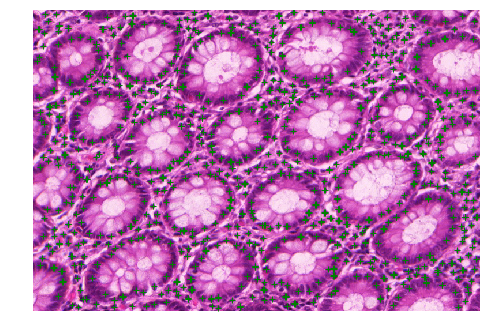
\includegraphics[height=1.5in]{figures/train_22_nuclei.png}
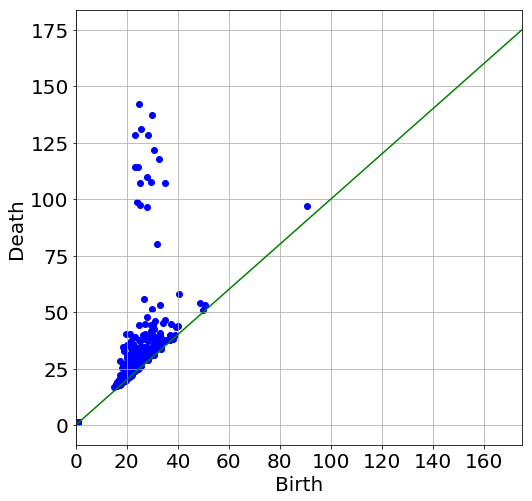
\includegraphics[height=1.5in]{figures/train_22_pd_bd.png}
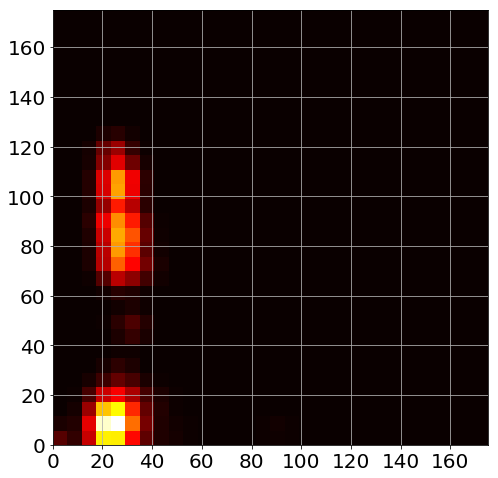
\includegraphics[height=1.5in]{figures/train_22_pi.png}
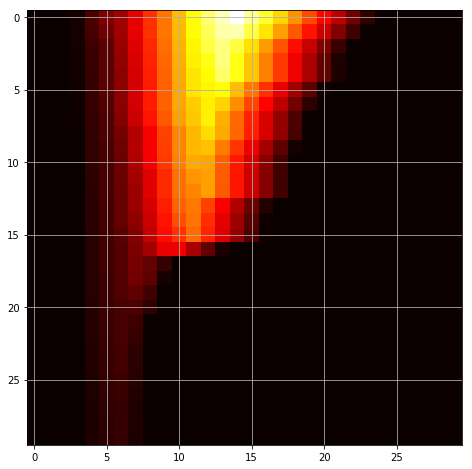
\includegraphics[height=1.5in]{figures/train_22_pl.png}\\
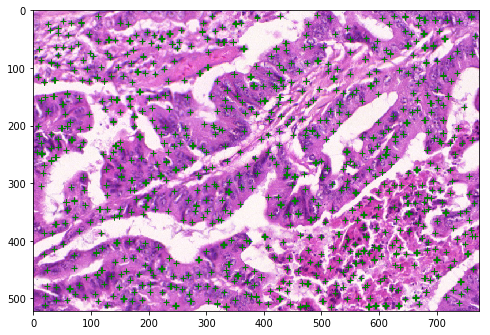
\includegraphics[height=1.5in]{figures/train_11_nuclei.png}
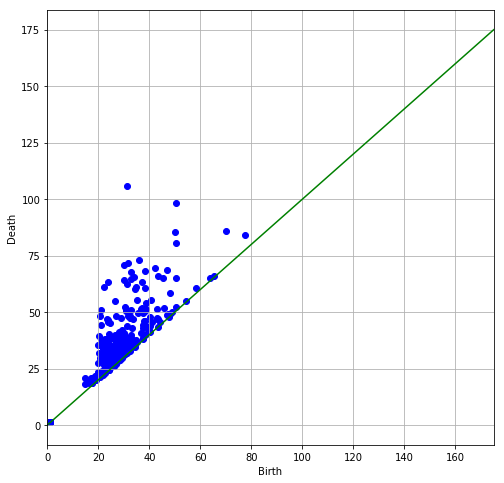
\includegraphics[height=1.5in]{figures/train_11_pd_bd.png}
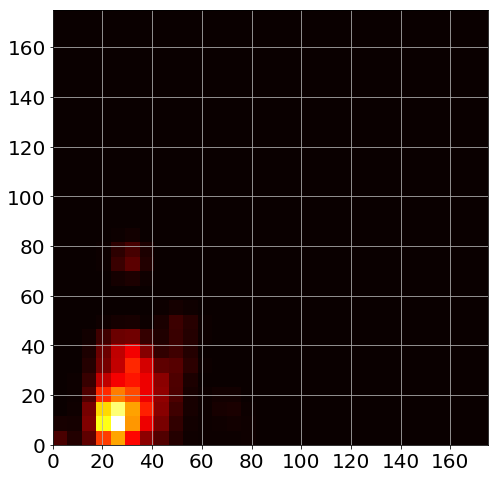
\includegraphics[height=1.5in]{figures/train_11_pi.png}
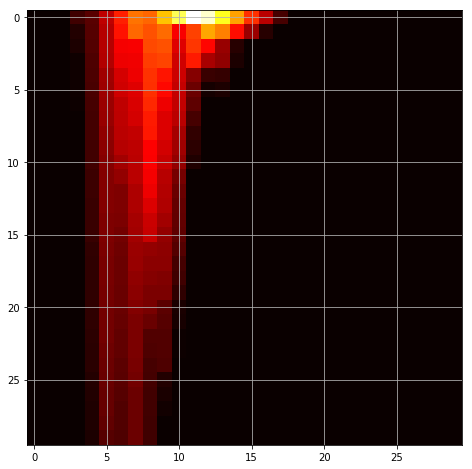
\includegraphics[height=1.5in]{figures/train_11_pl.png}
\caption{Illustration of persistent homology representations for sample benign and malignant images}
\label{fig:method_illustration}
\end{figure*}
%

\smallskip
\noindent \textbf{Persistence image (PI) representation:} Given a multi-set of $m$ birth-death points $BD=\{(b_i, d_i)\}_{i=1}^{m}$ from a PD, a linear transform $T(b, d) = (b, d-b)$ is applied to obtain a multi-set of birth-persistence points $BP=\{(b_i, p_i)\}_{i=1}^{m}$. Based on this, a 2D real-valued function $\rho_{bp} : \mathbb{R} \times \mathbb{R} \to \mathbb{R}$ called a persistence surface is defined as weighted sum of isotropic bi-variate gaussian/normal probability density functions $\mathcal{N}\left(x, y; \sigma^2\right)$ with variance $\sigma^2$ centered at each of the birth-persistence pairs as follows:
\begin{equation}
\rho_{bp}(x, y) = \sum_{i=1}^{m} w(b_i,p_i) * \mathcal{N}\left(x - b_i, y - p_i; \sigma^{2}\right)
\end{equation}
where $w(b, p)$ is a weighting function critical to the stability of the persistence surface. A natural choice is to pick a weighting function that assigns higher weights to points with higher persistence values. However, in certain applications, points of medium persistence may be more important. To allow this, the weighting function is defined more generally as a piece-wise linear function as follows:
\begin{equation}
w(b, p; c) = \left\{\begin{array}{ll}
 0 & if \; p \leq 0\\ 
 p / c & if \; p \leq c\\ 
 1 & otherwise
\end{array}\right.    
\end{equation}
where $c$ is the persistence value of the most important topological feature. Lastly, the persistence image is generated by defining a discrete grid in the domain of the 2D persistence surface function $\rho_{bp}(x, y)$ and computing its integral in each grid box. In case the birth values of all the points is equal to zero, as is often the case with the 0-dimensional homology group $H_0$ tracking the set of connected components, then both the persistence surface and persistence image can be represented compactly in 1D.  

\section{Method}
\label{sec:method}
In this section, we present the theory underlying the proposed method along with visual illustrations of intermediate results to help understand the underlying concepts. 

\smallskip
\noindent \textbf{Detect nuclei centroids:} Given a histology image, we first pre-process it using the color normalization method of Reinhard\etal~\cite{Reinhard2001}. Next, we use the unsupervised color deconvolution method of Macenko\etal~\cite{Macenko2009} to seperate out the nuclear stain. Next, we use the minimum cross entropy thresholding method of Li\etal~\cite{Li1998} to segment the nuclear foreground. Lastly, we use a fast difference-of-gaussian implementation of the scale-adaptive multiscale Laplacian-of-Gaussian filter proposed by Al-Kofahi\etal~\cite{Al-Kofahi2010} to detect the nuclear centroids. 

\smallskip
\noindent \textbf{Extract topological features using persistent homology:} Considering the set of nuclear centroid coordinates as a point cloud, we compute the persistence diagram of its Vectoris-rips filtration for the homological dimension-1 corresponding to 2D loops. Next, from the persistence diagram, we compute persistence landscape and persistence image representations as described in Section~\ref{sec:background} and use them as features encoding the underlying topological structure of the data. 

\smallskip
\noindent \textbf{Train machine learning model for cancer grading:}

\section{Results}
\label{sec:results}
We used the MICCAI 2015 Gland Segmentation Challenge Contest dataset~\cite{Sirinukunwattana2017} to develop and validate the proposed method. This dataset contains a total of 165 images derived from 16 hematoxylin-eosin stained histological sections of stage T3 and T4 colorectal adenocarcinoma digitized using a Zeiss MIRAX MIDI SlideScanner with a pixel resolution of $0.620 \mu m$ equivalent to a 20x objective magnification. An expert pathologist delineated the boundary of all the glands in each image and graded the image as either $benign$ or $malignant$ based on the overall glandular architecture. The dataset is divided into two parts: a training set of 85 images (37 benign, 48 malignant) and a test set of 80 images (37 benign, 43 malignant).

\begin{table}[h]
\centering
\begin{tabular}{|l|c|c|}
\hline
 & \textbf{Accuracy} & \textbf{AUC} \\ \hline
Persistence image features & 90 &  \\ \hline
Persistence landscape features & 86 &  \\ \hline
All persistence homology features &  &  \\ \hline
Cell graph features &  &  \\ \hline
\end{tabular}
\caption{Benign vs Malignant classification performance using different feature sets}
\label{tab:cancer_diagnosis_result}
\end{table}


\section{Conclusion}
\label{sec:conclusion}

Analysis of colorectal histology present significant challenges, since the tissue is highly anisotropic, and different cutting planes can reveal vastly different patterns.

% References
\bibliographystyle{IEEEbib}
\bibliography{refs}

\end{document}
